\documentclass[11pt]{article}
\usepackage[utf8]{inputenc}
\usepackage[T1]{fontenc}
\usepackage{minted}
\usepackage{graphicx}
\usepackage{hyperref}
\usepackage{CJKutf8}

\author{Student: Sean Wang, szw87 \\ Professor: Mohit Tiwari, Antonio Espinoza \\ Department of Electrical \& Computer Engineering \\ The University of Texas at Austin}
\date{\today}
\title{EE379K Enterprise Network Security Lab 3 Report}
\hypersetup{
 pdfauthor={Student: Sean Wang, szw87 \\ Professor: Mohit Tiwari, Antonio Espinoza \\ Department of Electrical \& Computer Engineering \\ The University of Texas at Austin},
 pdftitle={EE379K Enterprise Network Security Lab 3 Report},
 pdfkeywords={},
 pdfsubject={},
 pdfcreator={},
 pdflang={English}}

\begin{document}

\maketitle
\section*{Part 1 - APT Campaign Questions}
\subsection*{Exercise Set 1}
\begin{description}
  \item[1-1.] Dwell time is defined as the number of days that an attacker is present in a victim network. In other words, the
    time in days from the first evidence of compromise to detection. In the last year, the median dwell time has decrerased
    due to the fact that organizations are getting better at finding compromises internally, as well as the fact that clients
    have generally been improving data visiblity through better tools, resulting in faster responses. Median as a metric for
    dwell time can be good when a one number summary is needed, but it leaves out lots of information regarding the scale or
    complexity of the attacks.
  \item[1-2.] There are four new APT groups: APT37, APT38, APT39, and APT40. The primary mission of APT37, also known as "Reaper,"
    is to covertly gather intelligence to support North Korea's interests in military, politics, and economics, which is hypothesized due to their targeting of
    South Korean entities. Similarly, APT38, is a financially motivated group targeting financial institutions in support of
    the North Korean regime. APT39, on the other hand, is an Iranian cyber espionage group that seems to focus on monitoring,
    tracking, and surveilling specific people, collecting data to use for national priorities or for future campaigns. APT40,
    also known as "Periscope," is a Chinese cyber espionage group targeting countries important to China's "Belt and Road
    Initiative." They typically target sectors pertaining to engineering, transportation, and defense, especially those that
    overlap with maritime technology.
  \item[1-3.] APT37's known methods of initial compromise are phishing and strategic web compromise. Phishing is when the
    attacker attempts to get sensitive information using a diguise of a trustworthy entity. One such example is spear fishing,
    which occurs through emails or links. Defense against phishing attacks include using an antivirus to quarantine suspicious
    files or a system to scan incoming email attachments and remove any malicious ones. Additionaly, users can be trained to
    watch out for social engineering techniques and suspicious emails and links. On the other hand, strategic web compromises
    are when an attacker gets access into a system due to a user visiting a compromised website with malicious ads or injected
    code. One way to prevent this is to use network signatures to identify malware traffic. Additionally, proxies can be used
    to prevent the use of unauthorized external services through an enforced communication policy.
  \item[1-4.] Lack of investigation is problematic since it leaves out any information regarding the context of the malware
    and if a more in-depth analysis is needed. An in-depth analysis reveals much more about the system and the environment of
    the attack. Defenders can follow a more detailed analysis procedure to reveal much more information about attacks, including
    but not limited to: where it came from, how it attacked, and why it happened. The specific steps should be reviewed often
    as attack methods aren't stagnant, so defense against and analysis of attacks shouldn't be either. Poorly timed remediation
    is also problematic since organizations end up acting too fast to eradicate the attack, leaving some backdoors up in haste.
    As a result, the attack has not been fully eradicated and there is now no visibility of attacker activity either. Defenders
    can consider what evidence to keep and have more detailed guidelines so that attacker can be fully shut out.
\end{description}
\subsection*{Exercise Set 2}
\begin{description}
  \item[1-5.] The linked behavior, web service, is part of the command and control part of the APT lifecycle. This might be
    hard for defenders to detect since popular websites and social media can provide a lot of cover for the attack, since there
    is generally a prior connection to those sites before the compromise. In addition to common services providing noise, web
    service providers typically use SSL or TLS encryption, which gives these types of attacks another layer of protection.
  \item[1-6.] The web services used and number of times they are listed are shown below in Table \ref{table:services}.
    \begin{table}[h!]
      \centering
      \begin{tabular}{ c c }
      \hline
      Web Service & Examples \\
      \hline
      Social Networks & 8 \\
      Github & 8 \\
      Blogs & 7 \\
      Cloud Storage & 7 \\
      Google Apps & 7 \\
      Pastebin & 6 \\
      Microsoft TechNet & 4 \\
      RSS feeds & 2 \\
      Microsoft OneDrive & 2 \\
      Forums & 1 \\
      \hline
      \end{tabular}
      \caption{Table of web services used and the number of times listed.}
      \label{table:services}
    \end{table}
  \item[1-7.] The most prevalent web services are social networks, such as Twitter and AOL. Github is also a very common web
    service used in these attacks. To detect when these services are being used for malicious purposes, one can look for
    suspicious activity through packet capture analysis for communications that do not follow expected behavior. If the data
    is encrypted, then SSL/TLS inspection is also needed. Another method is to look for patterns, such as an uncommonly
    excessive amount of data flow or monitoring user activity.
\end{description}
\subsection*{Exercise Set 3}
\begin{description}
  \item[1-8.] Based on the APT41 report, it seems that an APT actor would be interested in targetting the video game industry
    most likely for personal financial gain and/or hobbyist interests. For example, by manipulating virtual currencies, they
    can prepare and sell accounts to sell in underground markets, or convert the virtual currency into real money through real
    money transfer purchases. Additionally, APT41 has utilized compromised digital certificates from video game studios in order
    to sign malware, since people tend to not check exactly what they download and install when they just want to play a game.
  \item[1-9.] Hammertoss is an effective tool that tries to prevent detection of malware by adding layers of complexity to
    obfuscate it, as well as mimicking normal user behavior. As a result, it tends to be very hard to detect. There are five
    stages that describe how it works. First, it looks for instructions on Twitter and is configured with certain restrictions
    to make its behavior blend in with normal traffic. Then, if that day's Twitter handle has been registered, the account
    tweets a URL and a hashtag, which tells at what offset the data begins and gives part of the encryption key needed to
    decrypt the data. Third, once it has obtained the Github URL from the second step, it downloads everything from that Github
    URL. Fourth, it searches the downloaded website contents for any images at least as large as the offset from step two, which
    contains hidden information that is then decrypted and executed. Finally, the encrypted info may contain instructions to
    execute a command in Powershell or some other file I/O or program execution. For example, it could upload sensitive info
    from the victim onto a cloud storage, which the attackers can easily access. All these layers and steps make it hard to 
    detect, especially since it employs legitimate web services that are widely used and implement SSL encryption which can
    disguise malicious traffic as normal traffic.
  \item[1-10.] Sudo caching is when an attacker abuses poor configurations of sudo's credential cache to see if the last entered
    credentials fall within the timeout range, which means that malware can then execute with elevated privileges without
    needing sudo credentials. This can be easily detected since sudo can also log all input and output using the \verb|LOG_INPUT| and
    \verb|LOG_OUTPUT| settings in \verb|/etc/sudoers|.
  \item[1-11.] MimiPenguin is a credential dumper, which means it retrieves and outputs the login and password of the current
    Linux user. It is part of the Credential Dumping stage of the APT lifecycle and can be used to move laterally to access
    restricted information.~\cite{cred_dump}
\end{description}
\section*{Part 2 - Fuzzing}
\begin{description}
  \item[2-1.] Notable behavior included crashing several times, likely due to some buffer overflow. This would look like
    Figure~\ref{fig:crash} on the Windows 7 VM. Some example commands that caused this were \verb|TRUN| followed by a random
    string of length 2100, \verb|KSTET| followed by a random string of length 100, or \verb|HTER| followed by a random string
    of length 4200.
    \begin{figure}[htbp]
      \centering
      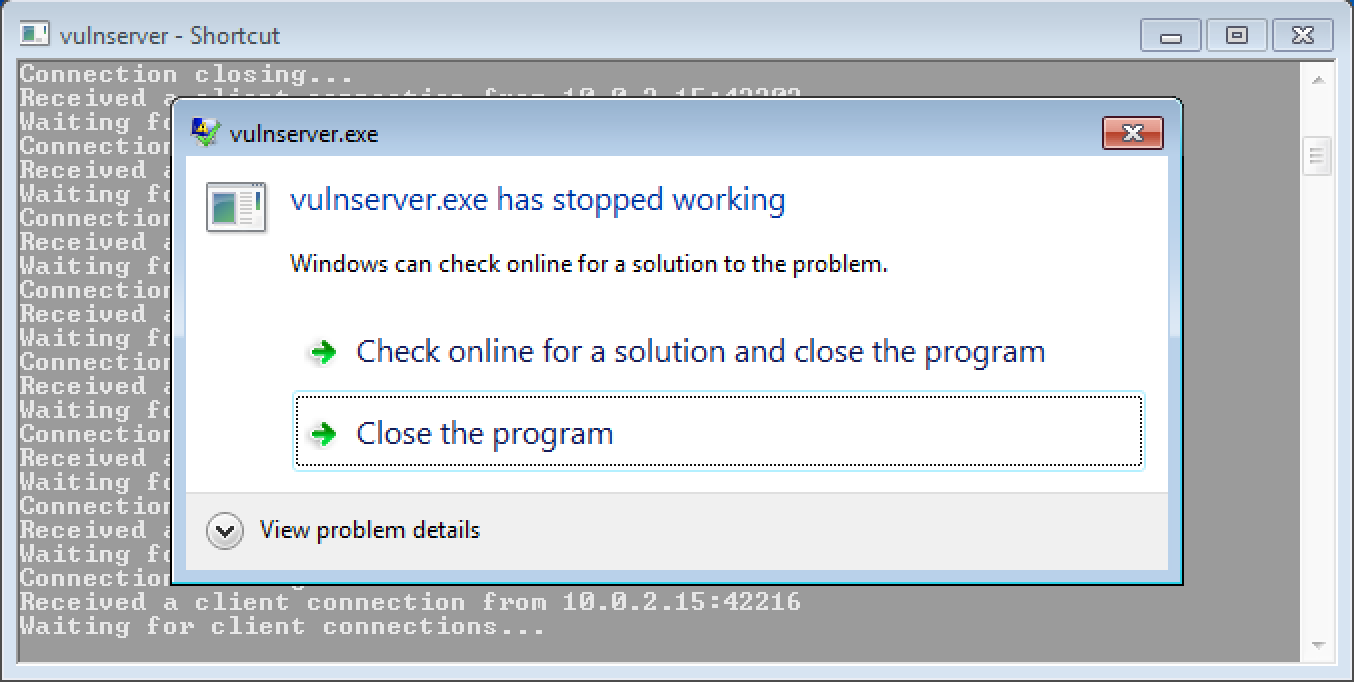
\includegraphics[width=1\linewidth]{./crash.png}
      \caption{vulnserver program crashing on Windows 7 VM.}
      \label{fig:crash}
    \end{figure}
  \item[2-2.] The server crash was likely due to a buffer overflow of the second argument. In the case of the \verb|KSTET|
    command, the second argument was a string of length 100 of random characters. This can be exploited by overwriting values
    on the stack and cause the program to execute some arbitrary code instead of functioning properly.
\end{description}
\section*{Part 3 - Exploitation}
\begin{description}
  \item[3-1.] The exploit is using HTTP.
  \item[3-2.] The Authorization header contains the payload.
  \item[3-3.] The HTTP Authorization request header is used to store encrypted credentials to authenticate a user agent with a
    server. The payload is encoded using Basic (base64) and, once decoded, results in a hexdump of
    \verb|0000 02 eb 61 a2 b8 b3 6a d8  a8|.
  \item[3-4.] 1012 bytes of overflow to the buffer is required before EIP is overwritten. In this case, it is being overwritten
    with the target return address, \verb|0x0040ae0f|.
  \item[3-5.] The above value returns to the exploit code.
  \item[3-6.] The Space variable has the value 600 and specifies how many bytes are given for the payload to reside in. Larger
    values could possibly cause corruption or truncation of the exploit.
  \item[3-7.] The exploit's exit function is 'thread' and this impacts the stability of the vulnerable program after the exploit
    is sent.~\cite{metasploit}
  \item[3-8.] The CVE number for this exploit is \verb|CVE-2009-0183|.
  \item[3-9.] The CVSS base score for this exploit is 10. This metric is based off of the fact that it is easily exploitable
    and has high impact, since remote attackers can run any arbitrary code just using a long Authorization header in an HTTP
    request.~\cite{nvd}
  \item[3-10.] The command \verb|getuid| shows the current user as \verb|victimbox\class|.
  \item[3-11.] The command \verb|getwd| shows the current directory as \\\verb|C:\Program Files\Free Download Manager|.
  \item[3-12.] The command \verb|sysinfo| shows the OS kernel and build version as \verb|Windows 7 (6.1 Build 7601)|.
  \item[3-13.] The commands \verb|getpid| and \verb|ps| show that the process being executed has name \verb|fdmwi.exe| and PID \verb|2192|.
  \item[3-14.] The command \verb|ifconfig| shows that the victim has 3 network interfaces and the MAC address of the one that is
    connected to is \\\verb|08:00:27:68:ed:0d|.
  \item[3-15.] Trying to access \verb|C:\Users\admin| results in an error saying that access has been denied, as shown below in
    Figure~\ref{fig:admin_dir}.
    \begin{figure}[htbp]
      \centering
      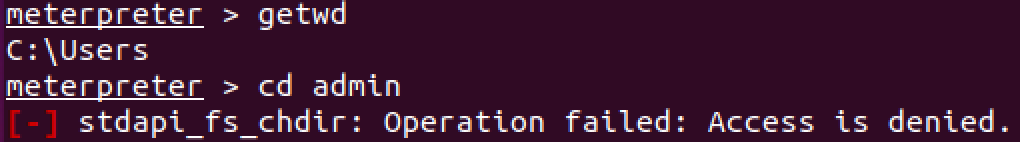
\includegraphics[width=1\linewidth]{admin_dir.png}
      \caption{Access denied to admin's user directory.}
      \label{fig:admin_dir}
    \end{figure}
  \item[3-16.] Running \verb|getsystem| results in another error saying that access has been denied, as shown below in
    Figure~\ref{fig:getsystem}. This is because Windows 7 is blocking the current user with normal user privileges from
    escalating privileges directly due to the User Account Control module.
    \begin{figure}[htbp]
      \centering
      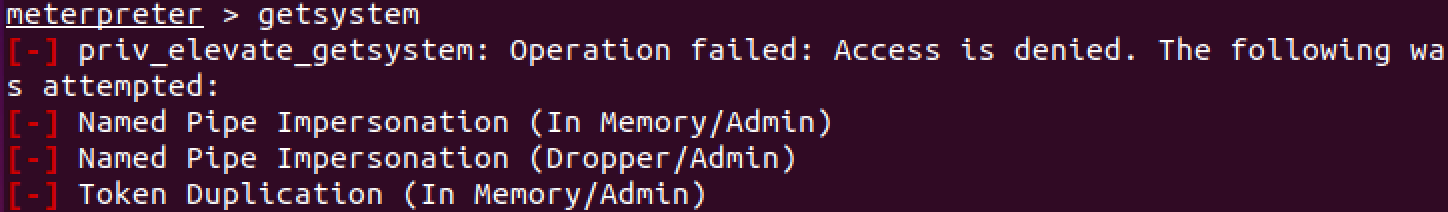
\includegraphics[width=1\linewidth]{./getsystem.png}
      \caption{Access denied to attempt to become SYSTEM user.}
      \label{fig:getsystem}
    \end{figure}
  \item[3-17.] Using the exploit shown in Figure~\ref{fig:esc_exploit} to open another meterpreter session, \verb|getuid| now
    returns \verb|NT AUTHORITY\SYSTEM| as the current user.
    \begin{figure}[htbp]
      \centering
      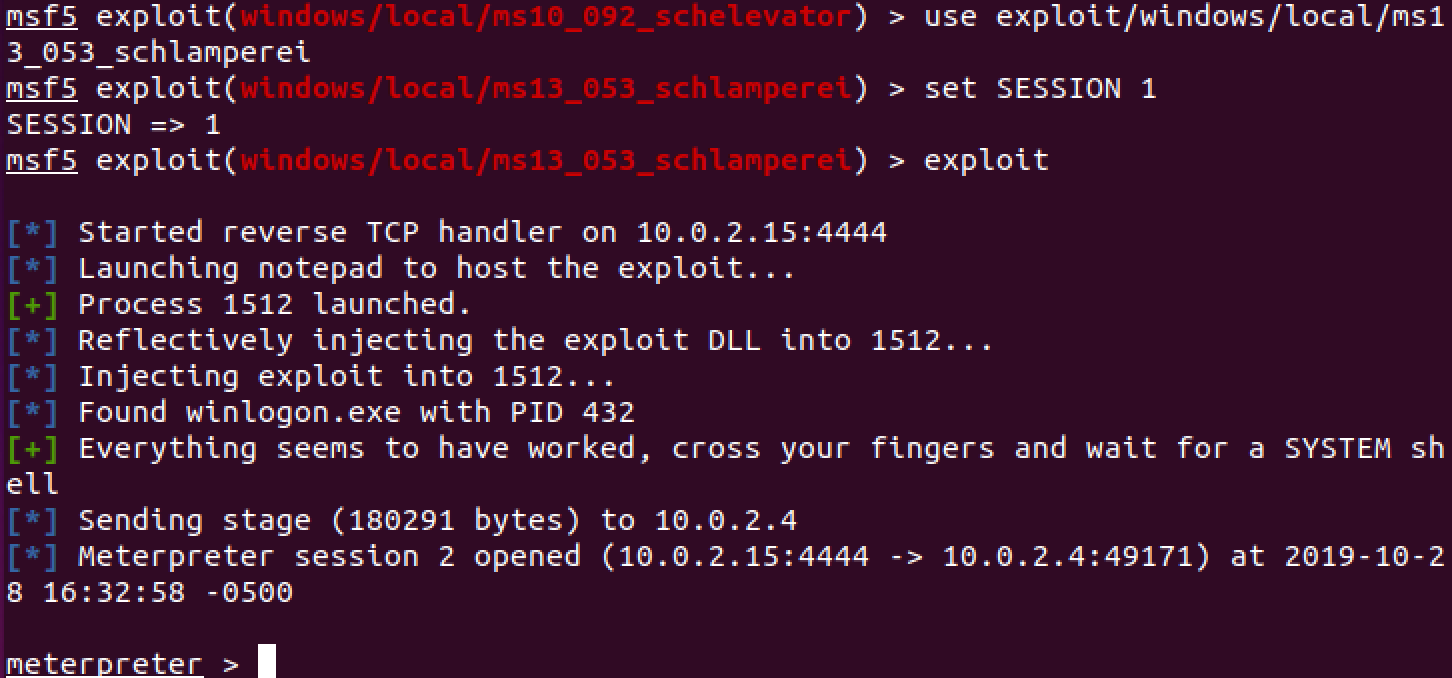
\includegraphics[width=1\linewidth]{./exploit.png}
      \caption{Exploit used to open an escalated session.}
      \label{fig:esc_exploit}
    \end{figure}
  \item[3-18.] The privilege escalation method used was \verb|Schlamperei|, as can be seen in Figure~\ref{fig:esc_exploit}.
  \item[3-19.] The commands \verb|getpid| and \verb|ps| now show that the current process is \verb|winlogon.exe| with PID \verb|432|.
  \item[3-20.] After getting the hashed passwords using \verb|hashdump|, with output shown in Figure~\ref{fig:hashdump}, the passwords
    were cracked by pasting them into https://crackstation.net/~\cite{crack}.
    \begin{figure}[htbp]
      \centering
      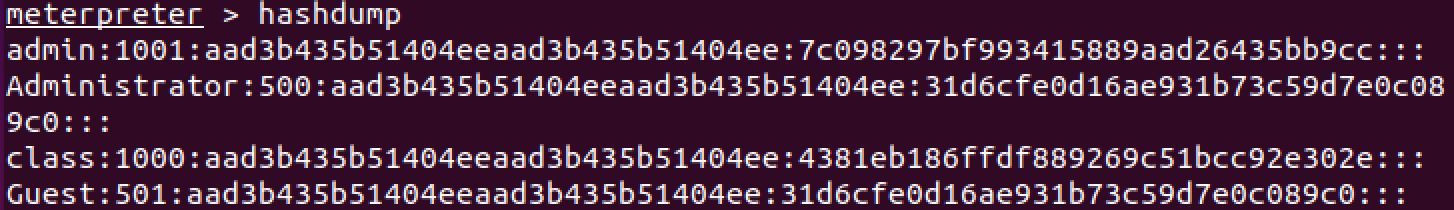
\includegraphics[width=1\linewidth]{./hashdump.png}
      \caption{Output of hashdump command.}
      \label{fig:hashdump}
    \end{figure}
  \item[3-21.] Decrypting admin's NTLM Hash shows that admin's password is \verb|iloveponies|.
  \item[3-22.] Using the elevated session, which can go into \verb|C:\Users\admin|, the contents of \verb|secret.txt| are shown
    below in Figure~\ref{fig:secret}.
    \begin{figure}[htbp]
      \centering
      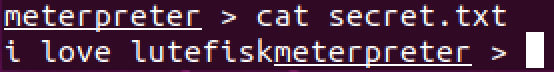
\includegraphics[width=.6\linewidth]{./secret.png}
      \caption{Contents of admin's secret.txt file.}
      \label{fig:secret}
    \end{figure}
\end{description}
\bibliography{bibliography}
\bibliographystyle{ieeetr}
\end{document}
